\chapter{Persamaan Schrödinger dalam Tiga Dimensi}\label{ch:b3:schrodinger-three-dimensions}

Layar televisi modern bersinar berkat kristal yang begitu kecil
sehingga \emph{ukurannya}lah yang menetapkan warnanya: sebutir
kadmium-selenida selebar empat nanometer bersinar merah, sedangkan zat
yang sama pada dua nanometer bersinar biru kehijauan. Tak ada yang
berbeda dalam kimianya --- hanya ukuran kotak yang mengurung
elektronnya. Jilid Tahun 2 berakhir dengan mekanika kuantum dalam satu
dimensi: fungsi gelombang pada sebuah garis, sumur, penghalang dan
penerowongan. Tetapi elektron hidup dalam tiga dimensi, dan langkah dari
garis ke ruang membawa fisika yang sungguh baru: peluang mengalir
sebagai arus melalui ruang, energi sebuah kotak menumpuk dengan
\emph{degenerasi} yang membocorkan simetrinya, keadaan harus
\emph{dicacah} --- pencacahan yang kelak menjalankan seluruh fisika
statistik --- dan soal berbentuk bola tereduksi, pada bentuk paling
sederhananya, menjadi persamaan satu dimensi yang menyamar pada
jejarinya. Bab ini mengambil langkah tersebut, dengan titik pusatnya
adalah titik kuantum sebuah televisi dan inti teringan di alam.

\section{Fungsi gelombang dalam ruang}

\begin{definition}[Fungsi gelombang dan peluang dalam tiga dimensi]\label{def:b3:schrodinger-three-dimensions:psi3d}
\index{fungsi gelombang!tiga dimensi}
Keadaan sebuah partikel adalah medan kompleks $\psi(\vect r, t)$ dengan
kaidah Born
\[
\dd\mathcal P = |\psi(\vect r, t)|^2\,\dd^3r , \qquad
\int|\psi|^2\,\dd^3r = 1 ,
\]
dan perkembangannya adalah persamaan Schrödinger dengan Laplacian
menggantikan turunan keduanya:
\[
\iu\hbar\,\frac{\partial\psi}{\partial t}
 = -\frac{\hbar^2}{2m}\,\Delta\psi + V(\vect r)\,\psi ,
\qquad
\Delta = \frac{\partial^2}{\partial x^2} +
\frac{\partial^2}{\partial y^2} + \frac{\partial^2}{\partial z^2} .
\]
Segala sesuatu yang ditegakkan jilid Tahun 2 bertahan kata demi kata:
kelinearan dan superposisi, keadaan stasioner
$\varphi(\vect r)\,\eu^{-\iu Et/\hbar}$ dengan
$-\tfrac{\hbar^2}{2m}\Delta\varphi + V\varphi = E\varphi$, dan
operator momentum, yang kini menjadi gradien $\hat{\vect p} =
-\iu\hbar\vect\nabla$.
\end{definition}

\begin{proposition}[Peluang mengalir: arusnya]\label{prop:b3:schrodinger-three-dimensions:current}
\index{arus peluang}
Kerapatan $\rho = |\psi|^2$ memenuhi persamaan kesinambungan,
\[
\frac{\partial\rho}{\partial t} + \operatorname{div}\vect\jmath = 0 ,
\qquad
\vect\jmath = \frac{\hbar}{m}\,
\operatorname{Im}\big(\psi^*\vect\nabla\psi\big) :
\]
peluangnya kekal secara setempat, diangkut oleh arus
$\vect\jmath$ --- untuk gelombang bidang $A\eu^{\iu\vect k\cdot\vect r}$,
$\vect\jmath = |A|^2\hbar\vect k/m = \rho\vect v$, yakni aliran seragam;
untuk $\varphi$ bernilai real mana pun, $\vect\jmath = \vect 0$:
keadaan stasioner terikat tidak membawa aliran neto.
\end{proposition}

\begin{proof}
Seperti dalam satu dimensi: $\partial_t(\psi^*\psi)$ dari persamaannya
dan konjugatnya; suku potensialnya saling meniadakan, dan $(\iu\hbar/2m)
(\psi^*\Delta\psi - \psi\Delta\psi^*) =
-\operatorname{div}\big[(\hbar/m)\operatorname{Im}(\psi^*\vect\nabla
\psi)\big]$ menurut aturan hasil kali untuk divergensinya.
\end{proof}

\begin{omfigure}
\begin{tikzpicture}[font=\small, >=Stealth]
  % plane wave current
  \begin{scope}
    \foreach \y in {0.3,0.9,1.5,2.1}
      \foreach \x in {0.2,1.2,2.2,3.2}
        \draw[->, omDef] (\x,\y) -- (\x+0.62,\y);
    \foreach \x in {0.55,1.55,2.55,3.55}
      \draw[omExo!60, dashed] (\x,-0.05) -- (\x,2.45);
    \node at (1.95,-0.62) {gelombang bidang: arus seragam $\rho\vect v$};
  \end{scope}
  % vortex-free bound state
  \begin{scope}[xshift=7.6cm]
    \draw[omThm, thick] (1.7,1.2) circle (1.35);
    \draw[omThm!50, thick] (1.7,1.2) circle (0.75);
    \node[omThm] at (1.7,1.2) {$\varphi$ real};
    \node at (1.85,-0.62) {keadaan terikat: $\vect\jmath = \vect 0$ di mana-mana};
  \end{scope}
\end{tikzpicture}

{\small \omterm{prop:b3:schrodinger-three-dimensions:current}{Arus peluang}: gelombang berjalan mengangkut kerapatannya
bagaikan fluida; fungsi gelombang yang real (terikat, stasioner) diam di
tempat --- awan elektron atom tidak beredar kecuali keadaannya kompleks.}
\end{omfigure}

\section{Kotak, degenerasi, dan pencacahan keadaan}

\begin{theorem}[Pemisahan variabel]\label{thm:b3:schrodinger-three-dimensions:separation}
\index{pemisahan variabel}
Jika potensialnya terpisah sebagai $V = V_1(x) + V_2(y) + V_3(z)$,
keadaan stasionernya dapat diambil sebagai hasil kali
$\varphi(\vect r) = \varphi_1(x)\,\varphi_2(y)\,\varphi_3(z)$, dengan
tiap faktornya menyelesaikan soal satu dimensinya sendiri, dan
energinya \emph{dijumlahkan}: $E = E_1 + E_2 + E_3$. Dalam kasus
semacam itu, tiga dimensi adalah satu dimensi sebanyak tiga kali.
\end{theorem}

\begin{proof}
Masukkanlah hasil kalinya ke persamaan stasionernya lalu bagilah dengan
$\varphi$: jumlah tiga bentuk bervariabel tunggal sama dengan tetapan
$E$, sehingga masing-masingnya tetap secara terpisah. Bahwa setiap
keadaan merupakan superposisi hasil kali semacam itu adalah kelengkapan
penyelesaian 1D-nya, yang diterima tanpa bukti.
\end{proof}

\begin{proposition}[Kotak kubus dan degenerasinya]\label{prop:b3:schrodinger-three-dimensions:box}
\index{degenerasi}
Dalam kotak bersisi $a$ berdinding tak tertembus, keadaannya diindeks
oleh tiga bilangan bulat positif,
\[
\varphi_{n_1n_2n_3} \propto
\sin\frac{n_1\pi x}{a}\sin\frac{n_2\pi y}{a}\sin\frac{n_3\pi z}{a} ,
\qquad
E = \frac{h^2}{8ma^2}\,(n_1^2 + n_2^2 + n_3^2) .
\]
Keadaan yang berbeda kini berbagi energi: aras $(2,1,1)$ hadir dalam
tiga salinan, karena $(1,2,1)$ dan $(1,1,2)$ merupakan keadaan yang
berbeda secara fisis dengan $E$ yang sama. \emph{Degenerasi} semacam itu
adalah tanda adanya simetri --- di sini, dapat dipertukarkannya ketiga
sumbu kotaknya; gepengkanlah kotaknya sedikit dan tripletnya terbelah.
\end{proposition}

\begin{proof}
Pemisahan dengan tiga sumur tak hingga jilid Tahun 2; energinya
dijumlahkan.
\end{proof}

\begin{omfigure}
\begin{tikzpicture}[font=\small]
  \draw[->] (0,0) -- (0,6.1);
  \node[anchor=south] at (0,6.1) {$E\,/\,\dfrac{h^2}{8ma^2}$};
  \foreach \e/\lab/\deg in {3/{(1,1,1)}/1, 6/{(2,1,1)}/3, 9/{(2,2,1)}/3,
      11/{(3,1,1)}/3, 12/{(2,2,2)}/1, 14/{(3,2,1)}/6}
    {\draw[very thick, omDef] (0.6,\e*0.42) -- (2.6,\e*0.42);
     \node[anchor=west] at (2.75,\e*0.42) {$\e$\quad\lab, degenerasi \deg};}
\end{tikzpicture}

{\small Aras terendah kotak kubus: energinya dalam satuan
$h^2/8ma^2$ beserta bilangan kuantumnya. Permutasi $n_i$ yang tidak sama
memberikan triplet dan sekstet berdegenerasi --- yakni sidik jari
simetri kubus.}
\end{omfigure}

\begin{proposition}[Mencacah keadaan]\label{prop:b3:schrodinger-three-dimensions:counting}
\index{kerapatan keadaan}
Banyaknya keadaan kotak berenergi di bawah $E$ adalah, untuk $E$ besar,
\[
N(E) \approx \frac{V}{6\pi^2}\Big(\frac{2mE}{\hbar^2}\Big)^{3/2} ,
\qquad V = a^3 :
\]
sebanding dengan volumenya dan dengan $E^{3/2}$. Setara dengan itu,
\omterm{def:b3:hamiltonian-mechanics:hamiltonian}{ruang fase} memuat satu keadaan kuantum tiap volume $h^3$ --- yakni sel
Bohr--Sommerfeld pada
\cref{ch:b3:hamiltonian-mechanics}, yang kini diturunkan. Satu
pencacahan inilah bahan mentah fisika statistik dan fisika zat padat di
bagian selanjutnya jilid ini: elektron dalam logam, foton dalam rongga,
dan pijar benda panas semuanya bermula di sini.
\end{proposition}

\begin{proof}
Keadaannya adalah titik kisi $(n_1, n_2, n_3)$ dalam oktan positif;
$E \le E_{\max}$ mempertahankan yang berada di dalam bola berjejari $R =
\sqrt{8ma^2E/h^2}$. Untuk $R$ besar, cacahnya sama dengan volume
oktannya $\tfrac18\cdot\tfrac43\pi R^3$; sulihkanlah. (Versi \omterm{def:b3:hamiltonian-mechanics:hamiltonian}{ruang
fasenya}: $N = \tfrac{V\cdot\frac43\pi p^3}{h^3}$ dengan $p = \sqrt{2mE}$ ---
bilangan yang sama.)
\end{proof}

\begin{example}[Sebuah logam, taksiran pertama]\label{ex:b3:schrodinger-three-dimensions:metal}
Tembaga menyediakan kira-kira satu elektron bergerak tiap atom, $n =
\qty{8.5e28}{m^{-3}}$. Mengisi keadaan kotaknya dua elektron masing-masing
(spin, \cref{ch:b3:spin-two-level}) sampai energi yang memuat semuanya
memberikan, dengan membalik pencacahannya, $E_{\text{F}}
\approx \qty{7}{eV}$ --- energi yang luar biasa besar dibandingkan
dengan kegelisahan termalnya ($k_{\text{B}}T \approx \qty{25}{meV}$):
bahkan pada suhu ruang elektron sebuah logam merupakan kerumunan yang
sangat kuantum. Kisah lengkapnya ada pada
\cref{ch:b3:electrons-in-solids}.
\end{example}

\begin{example}[Osilator isotropik]\label{ex:b3:schrodinger-three-dimensions:oscillator}
Untuk $V = \tfrac12 m\omega^2r^2 = \tfrac12 m\omega^2(x^2 + y^2 +
z^2)$, pemisahannya memberikan $E = (n_x + n_y + n_z + \tfrac32)\hbar\omega$:
aras $\tfrac32, \tfrac52, \tfrac72\hbar\omega\ldots$ dengan
degenerasi $1, 3, 6, 10, \dots$ --- yang tumbuh, tidak seperti pola tak
beraturan kotaknya, dengan keteraturan sempurna. Degenerasi tambahan di
luar yang dijelaskan permutasi sumbu menandakan simetri tersembunyi yang
\emph{lebih besar}; atom hidrogen kelak mengulangi muslihat itu secara
mengagumkan. Diisi dengan partikel berpasangan spin, kulit osilator ini
memuat $2,
8, 20, \dots$ --- hampiran pertama bagi ``bilangan sakti'' fisika inti
(\cref{ch:b3:nuclear-physics}).
\end{example}

\section{Soal berbentuk bola: muslihat gelombang s}

\begin{proposition}[Keadaan bersimetri bola]\label{prop:b3:schrodinger-three-dimensions:swave}
\index{s keadaan@keadaan $s$}\index{persamaan radial}
Untuk potensial sentral $V(r)$, carilah keadaan yang hanya bergantung
pada $r$ (yakni \emph{keadaan s}; kasus umumnya, dengan struktur
sudutnya, menunggu \cref{ch:b3:quantum-angular-momentum}). Dengan
menuliskan $\varphi(r) = u(r)/r$, fungsi $u$ memenuhi
\[
-\frac{\hbar^2}{2m}\,u'' + V(r)\,u = E\,u ,
\qquad u(0) = 0 :
\]
yakni \emph{tepat} persamaan Schrödinger satu dimensi pada setengah
garis, dengan dinding di titik asalnya. Setiap perkakas 1D jilid Tahun 2
--- sumur, penyesuaian, penerowongan --- berlaku kata demi kata bagi
soal berbentuk bola, dengan harga satu penyulihan.
\end{proposition}

\begin{proof}
Untuk $\varphi(r)$, Laplaciannya menyusut menjadi $\Delta\varphi =
\tfrac1r(r\varphi)'' = u''/r$; masukkanlah lalu kalikan dengan $r$.
Syarat $u(0) = 0$ menjaga $\varphi = u/r$ tetap berhingga di titik
asalnya; penormalannya adalah $\int_0^\infty|u|^2\dd r$ kali $4\pi$ ---
jadi $u$ adalah fungsi gelombang 1D yang sejati.
\end{proof}

\begin{example}[Deuteron: nyaris bukan inti]\label{ex:b3:schrodinger-three-dimensions:deuteron}
Deuteron --- satu proton, satu neutron --- adalah inti yang paling
sederhana: energi ikatnya $B = \qty{2.2}{MeV}$, mungil dibandingkan
skala inti. Sebagai model, tempatkanlah gerak nisbinya (massa tereduksi
$m_{\text{p}}/2$) dalam sumur bola berjangkauan $R = \qty{2.1}{fm}$ dan
berkedalaman $V_0$: persamaan $u$-nya adalah sumur 1D berhingga.
Menyesuaikan penyelesaian di dalam dan di luarnya menuntut kedalaman
minimum $V_0 > \pi^2\hbar^2/8\mu R^2
\approx \qty{23}{MeV}$ agar ada keadaan terikat \emph{sama sekali}, dan
menghasilkan kembali $B = \qty{2.2}{MeV}$ menuntut $V_0 \approx \qty{35}{MeV}$
(\cref{exo:b3:schrodinger-three-dimensions:10}): gaya kuat mengikat
deuteron hanya dengan kelonggaran sepuluh persen. Fungsi gelombangnya
merembes jauh ke luar sumurnya --- pasangan nukleonnya menghabiskan
sebagian besar waktunya di luar jangkauan gayanya --- dan tidak ada
keadaan terikat kedua: inti tersederhana kedua di alam, yaitu helium,
memerlukan nukleon ketiga.
\end{example}

\begin{omfigure}
\begin{tikzpicture}
  \begin{axis}[omaxis, axis x line=bottom, axis y line=left,
    width=11.2cm, height=5.6cm, xmin=0, xmax=8, ymin=-1.25, ymax=1.15,
    xlabel={$r$ (fm)}, ylabel={},
    xlabel style={at={(axis description cs:0.5,-0.1)}, anchor=north},
    xtick={2.1}, xticklabels={$R$}, ytick=\empty, clip=false]
    % well
    \draw[omExo, thick] (axis cs:0,-1.0) -- (axis cs:2.1,-1.0) --
      (axis cs:2.1,0) -- (axis cs:8,0);
    \node[omExo, font=\scriptsize, anchor=west] at (axis cs:0.12,-1.12) {$-V_0$};
    % energy level
    \draw[omThm, dashed] (axis cs:0,-0.063) -- (axis cs:8,-0.063);
    \node[omThm, font=\scriptsize, anchor=south west] at (axis cs:5.3,-0.05) {$E = -B$};
    % u(r): sin inside, exp outside, matched at R
    \addplot[omDef, very thick, domain=0:2.1, samples=50]
      {0.92*sin(deg(0.87*x))};
    \addplot[omDef, very thick, domain=2.1:8, samples=50]
      {0.888*exp(-0.232*(x-2.1))};
    \node[omDef, font=\scriptsize, anchor=west] at (axis cs:3.6,0.75) {$u(r)$: ekor eksponensial yang panjang};
  \end{axis}
\end{tikzpicture}

{\small Fungsi gelombang radial deuteron $u(r)$ dalam model sumur bola:
nyaris hanya seperempat osilasi yang muat di dalam sumurnya, dan
keadaannya bertahan berkat ekor yang menjangkau jauh melampaui jangkauan
gayanya --- sebuah inti yang terikat sebesar \qty{2.2}{MeV} dalam sumur
sedalam \qty{35}{MeV}.}
\end{omfigure}

\begin{method}[Soal tiga dimensi]\label{met:b3:schrodinger-three-dimensions:method}
(1) Potensialnya aditif ($V_1 + V_2 + V_3$)? Pisahkanlah; energinya
dijumlahkan; himpunlah degenerasinya menurut simetrinya. (2) Potensial
sentral, keadaan berbentuk bola? Sulihkanlah $\varphi = u/r$ lalu
pakailah kembali setiap hasil 1D dengan $u(0) = 0$. (3) Untuk mencacah
keadaan, berpikirlah dalam ruang $\vect n$ atau dalam \omterm{def:b3:hamiltonian-mechanics:hamiltonian}{ruang fase} dengan
satu keadaan tiap $h^3$ (tiap keadaan spin). (4) Arus: hitunglah
$\vect\jmath$ ketika aliran atau fluks berperan; ingatlah: fungsi
gelombang real $=$ tanpa arus. (5) Taksiran lebih dahulu: energi
pengurungan $\sim h^2/8mL^2$ tiap arah menetapkan skalanya, dari titik
kuantum sampai inti, sebelum satu persamaan pun diselesaikan.
\end{method}

\begin{omfigure}
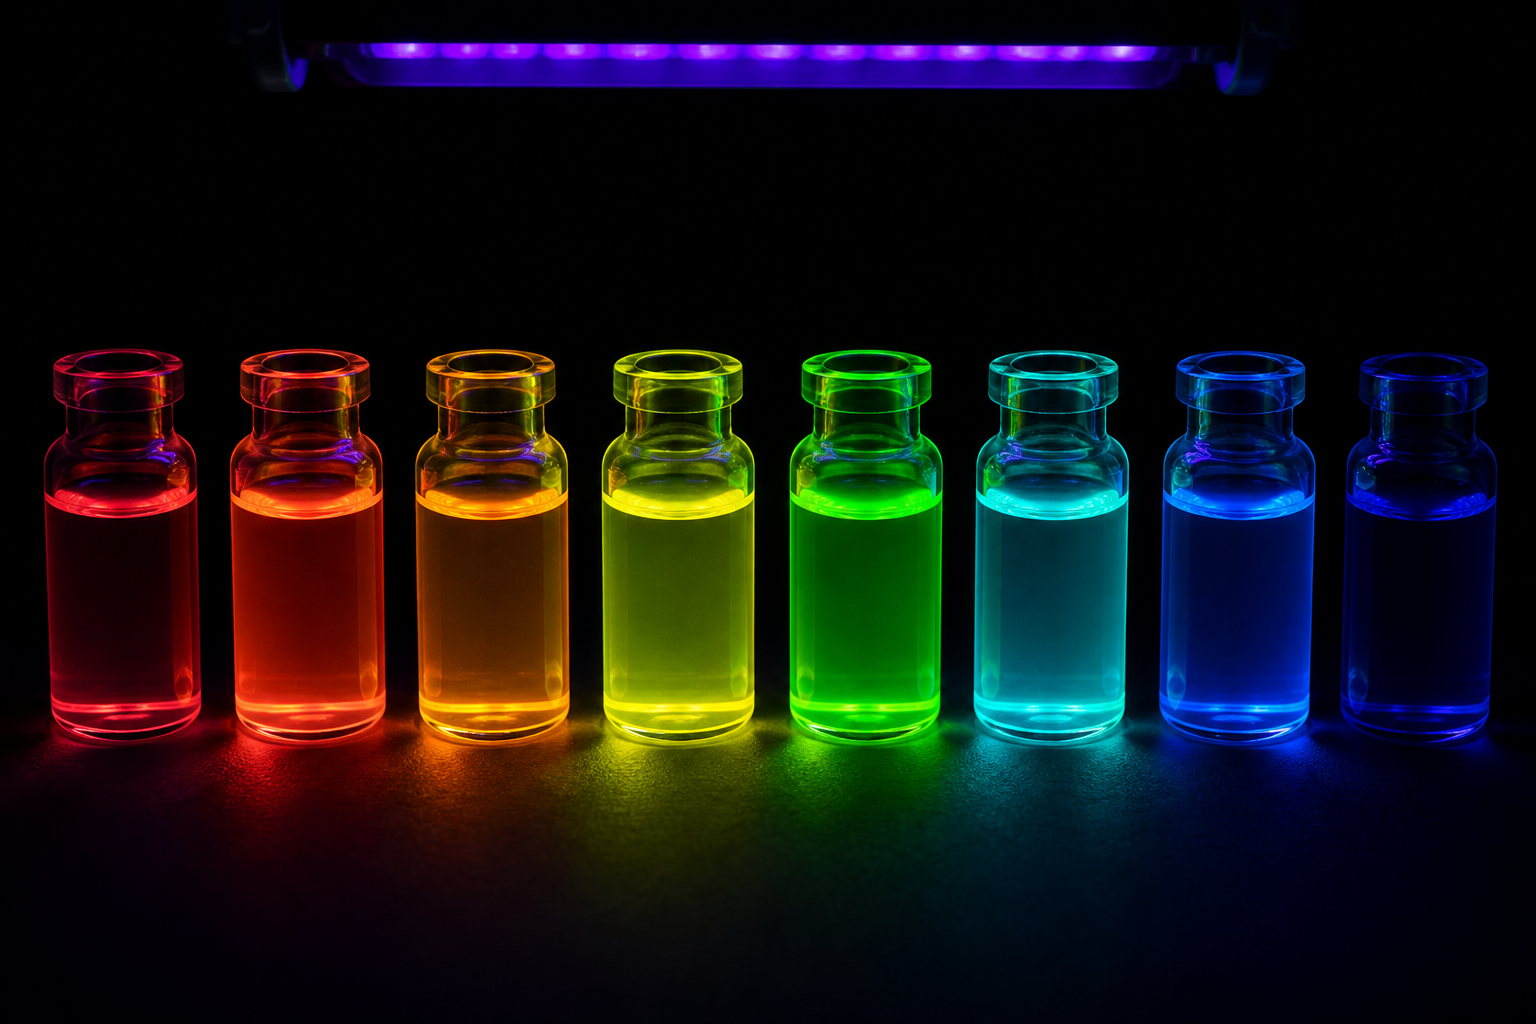
\includegraphics[width=0.58\linewidth]{images/book5/ai/b5-07-quantum-dot-vials.png}

{\small Titik kuantum di bawah cahaya ultraungu: semikonduktor yang sama, dalam kristal yang makin kecil, bersinar dari merah sampai biru. Warnanya ditetapkan oleh energi partikel-dalam-kotak pada bab ini --- pengurungan yang dapat Anda lihat.}
\end{omfigure}

\section{Latihan}

\begin{exercise}[$\star$]\label{exo:b3:schrodinger-three-dimensions:1}
Keadaan Gauss $\psi(\vect r) = A\,\eu^{-r^2/4\sigma^2}$. (a)
Normalkanlah ($\int_0^\infty x^2\eu^{-x^2}\dd x = \sqrt\pi/4$). (b)
Hitunglah $\langle r^2\rangle$ dan $\Delta x$ (keisotropannya
membantu). (c) Berapa $\vect\jmath$ untuk keadaan ini, dan mengapa? (d)
Kalikanlah dengan $\eu^{\iu\vect k_0\cdot\vect r}$: berapa kini $\langle\vect
p\rangle$ dan $\vect\jmath$?
\end{exercise}

\begin{exercise}[$\star$]\label{exo:b3:schrodinger-three-dimensions:2}
Untuk kotak kubus, daftarkanlah semua aras sampai $E = 15$ (dalam satuan
$h^2/8ma^2$) beserta degenerasinya. Lalu tunjukkanlah bahwa aras $27$
berdegenerasi \emph{melampaui} permutasinya: carilah kedua keluarga
bilangan kuantumnya, lalu katakanlah mengapa degenerasi ``kebetulan''
semacam itu tidak menyusul dari simetri kubusnya.
\end{exercise}

\begin{exercise}[$\star$]\label{exo:b3:schrodinger-three-dimensions:3}
Hitunglah arus $\vect\jmath$ untuk: (a) gelombang bidang
$A\eu^{\iu kx}$; (b) gelombang berdiri $A\sin kx$; (c) superposisi
$A(\eu^{\iu kx} + r\,\eu^{-\iu kx})$ dengan $r$ real --- tafsirkanlah
hasilnya sebagai fluks datang dikurangi fluks pantul; (d) keadaan
$A\,\eu^{\iu m\varphi}$ pada cincin berjejari $b$ (pakailah $|\vect\nabla|
= (1/b)\partial_\varphi$ di sana): sebuah arus yang beredar selamanya.
\end{exercise}

\begin{exercise}[$\star$]\label{exo:b3:schrodinger-three-dimensions:4}
Sebutir kristal titik kuantum mengurung pasangan elektron--lubang
bermassa efektif $\mu = 0.10\,m_{\text{e}}$; energi foton yang
dipancarkannya adalah celah ruahnya $E_{\text{g}} = \qty{1.74}{eV}$
ditambah energi pengurungan kotak bola, $\pi^2\hbar^2/2\mu R^2$. (a)
Hitunglah energi pengurungannya pada $R = \qty{3}{nm}$. (b) Berapa
panjang gelombang yang dipancarkannya? (c) Ke arah mana warnanya bergerak
ketika titiknya mengecil? (d) Mengapa kadmium selenida ruah ($R$ besar)
menunjukkan satu warna tetap saja?
\end{exercise}

\begin{exercise}[$\star\star$]\label{exo:b3:schrodinger-three-dimensions:5}
Partikel pada cincin (jejari $b$, koordinat $\varphi$): keadaan
stasionernya adalah $\psi_m = \eu^{\iu m\varphi}/\sqrt{2\pi}$. (a)
Mengapa $m$ harus bilangan bulat? (b) Tunjukkanlah $E_m = \hbar^2m^2/2mb^2$ ---
hati-hati dengan kedua $m$-nya: tuliskanlah $E_m = \hbar^2 m^2/2Mb^2$ untuk massa
$M$ --- lalu perhatikanlah bahwa tiap aras dengan $m \neq 0$ berdegenerasi ganda:
simetri apa yang memasangkan $+m$ dengan $-m$? (c) Hitunglah arus
$\psi_m$ beserta momen magnetik ``orbital'' yang menyertainya jika
partikelnya bermuatan $q$. (d) Keenam elektron bergerak benzena hidup
pada cincin berjejari $b \approx \qty{1.4}{\angstrom}$: perkirakanlah
energi foton eksitasi terizinkan pertamanya ($m = \pm1 \to \pm2$) lalu
bandingkanlah dengan serapan ultraungu benzena di dekat \qty{180}{nm} ---
satu cincin, tanpa kimia.
\end{exercise}

\begin{exercise}[$\star\star$]\label{exo:b3:schrodinger-three-dimensions:6}
Degenerasi osilator isotropik. (a) Tunjukkanlah bahwa banyaknya rangkap
tiga dengan $n_x + n_y + n_z = n$ adalah $(n+1)(n+2)/2$. (b)
Daftarkanlah pengisian kulitnya untuk $n = 0$ sampai $3$, dilipatduakan
karena spinnya. (c) Tunjukkanlah bahwa pengisian kumulatifnya $2, 8, 20, 40, \dots$:
ketiga yang pertama cocok dengan bilangan nukleon ``sakti'' yang
bertambah mantap dalam fisika inti --- apa yang disarankan kegagalannya
pada $40$ (yang sakti sesungguhnya: $28$, $50$) tentang potensial
intinya? (d) Mengapa pola aras kotaknya yang tak beraturan, tidak
seperti pola osilatornya, tidak menghasilkan struktur kulit yang kuat?
\end{exercise}

\begin{exercise}[$\star\star$]\label{exo:b3:schrodinger-three-dimensions:7}
Sumur bola tak hingga (jejari $R$): dengan memakai muslihat gelombang $s$,
(a) carilah aras $E_n = n^2\pi^2\hbar^2/2MR^2$ beserta fungsi gelombangnya
$u_n$; (b) hitunglah $E_1$ untuk sebuah nukleon ($Mc^2 =
\qty{939}{MeV}$) dalam $R = \qty{5}{fm}$ (pakailah $\hbar c =
\qty{197.3}{MeV.fm}$); (c) bandingkanlah dengan jarak antararas nukleon
terukur yang beberapa MeV pada inti sedang; (d) di manakah partikelnya
paling mungkin ditemukan dalam keadaan dasarnya --- hitunglah maksimum
$|u_1|^2$, lalu pertentangkanlah dengan jawaban kotak 1D untuk $|\varphi|^2$.
\end{exercise}

\begin{exercise}[$\star\star$]\label{exo:b3:schrodinger-three-dimensions:8}
Mencacah elektron dalam logam. (a) Dari
\cref{prop:b3:schrodinger-three-dimensions:counting} dengan dua keadaan
spin, tunjukkanlah bahwa mengisi $N$ elektron dalam volume $V$ mencapai
energi Fermi
\[
E_{\text{F}} = \frac{\hbar^2}{2m_{\text{e}}}\,(3\pi^2n)^{2/3} ,
\qquad n = N/V .
\]
(b) Hitunglah untuk tembaga. (c) Hitunglah laju Fermi dan suhu Fermi
$E_{\text{F}}/k_{\text{B}}$ yang bersesuaian. (d) Dalam satu kalimat:
mengapa elektronnya tidak semuanya duduk di keadaan dasar, dan asas
mana (yang dipratayangkan di sini, dibuktikan dalam
\cref{ch:b3:identical-particles}) yang melarangnya?
\end{exercise}

\begin{exercise}[$\star\star$]\label{exo:b3:schrodinger-three-dimensions:9}
Kedalaman minimum sumur bola. Untuk sumur berhingga ($-V_0$ untuk
$r < R$), keadaan dasar gelombang $s$-nya mempunyai $u = \sin kr$ di
dalam dan $\eu^{-\kappa r}$ di luarnya. (a) Tuliskanlah $k$ dan $\kappa$
beserta syarat penyesuaiannya $k\cot kR = -\kappa$. (b) Tunjukkanlah
bahwa keadaan terikat pertama kali muncul ketika $kR = \pi/2$ tepat pada
$E = 0$, sehingga $V_{0,\min} = \pi^2\hbar^2/8MR^2$. (c) Hitunglah untuk
deuteronnya ($M \to \mu = m_{\text{p}}/2$, $R = \qty{2.1}{fm}$). (d)
Pertentangkanlah dengan satu dimensi, tempat sumur sedangkal apa pun
mengikat: apa yang diubah dinding $u(0) = 0$ itu secara fisis?
\end{exercise}

\begin{exercise}[$\star\star\star$]\label{exo:b3:schrodinger-three-dimensions:10}
Deuteron, diselesaikan. Dengan $\mu c^2 = \qty{469}{MeV}$, $R =
\qty{2.1}{fm}$, $B = \qty{2.22}{MeV}$: (a) hitunglah $\kappa$ dari $B$
beserta panjang ekornya $1/\kappa$; (b) tuliskanlah syarat
penyesuaiannya lalu tunjukkanlah bahwa ia menjadi $\cot kR = -\kappa/k$
dengan $k$ ditetapkan oleh $V_0 - B$; (c) selesaikanlah untuk $V_0$
(dengan lelaran: mulailah dari $kR \approx 0.6\pi$) lalu berikanlah
$V_0$ sampai MeV terdekat; (d) hitunglah peluang bahwa kedua nukleonnya
berjarak lebih dari $R$ (integralkanlah ekornya), lalu berilah ulasan
tentang ``sebuah inti yang hidup sebagian besar di luar gayanya sendiri''.
\end{exercise}

\begin{exercise}[$\star\star\star$]\label{exo:b3:schrodinger-three-dimensions:11}
Ehrenfest dan kesinambungan dalam tiga dimensi. (a) Buktikanlah
$\dd\langle\vect r\rangle/\dd t = \langle\vect p\rangle/m$ dari
persamaan kesinambungannya (integralkanlah $\vect r\,\partial_t\rho$
secara parsial). (b) Buktikanlah $\dd\langle\vect p\rangle/\dd t =
-\langle\vect\nabla V\rangle$. (c) Pada syarat apa atas $V$ maka
$\langle\vect r\rangle$ mengikuti lintasan klasiknya secara tepat? (d)
Berikanlah satu kasus nyata yang tidak demikian (misalnya paket yang
terbelah oleh potensial celah ganda) lalu jelaskanlah apa yang kemudian
diperikan rata-ratanya.
\end{exercise}

\begin{exercise}[$\star\star\star$]\label{exo:b3:schrodinger-three-dimensions:12}
Mengapa atom tidak runtuh. Modelkanlah keadaan dasar hidrogen dengan
fungsi coba $\psi \propto \eu^{-r/a}$ dengan $a$ yang dapat diatur. (a)
Dengan menerima $\langle E_k\rangle = \hbar^2/2m_{\text{e}}a^2$ dan
$\langle E_p\rangle = -e^2/4\pi\varepsilon_0a$, jelaskanlah asal usul
tiap penyekalaannya. (b) Minimumkanlah $E(a)$ lalu tunjukkanlah bahwa
optimumnya adalah jejari Bohr, dengan $E = \qty{-13.6}{eV}$. (c) Mengapa
memperkecil $a$ di bawah optimumnya justru \emph{menaikkan} energinya,
padahal potensialnya makin dalam? (d) Argumen yang sama dengan $1/r$
digantikan tarikan gravitasi antara elektron dan proton: carilah
``jejari Bohr gravitasi''nya lalu simpulkanlah mengapa gravitasi tidak
membangun atom.
\end{exercise}

\section{Soal: Warna sebuah titik kuantum}

\begin{problem}[{Soal akhir pekan --- merekayasa cahaya dengan menghitung
nanometer}]\label{pb:b3:schrodinger-three-dimensions:1}
Hadiah Nobel Kimia 2023 diberikan bagi penemuan dan sintesis titik
kuantum: kristal yang begitu kecil sehingga energi partikel-dalam-kotak
pada bab ini menetapkan warnanya, yang kini bersinar di layar televisi
dan menandai molekul dalam sel hidup. Soal ini merancang layar titik
kuantum dari persamaan Schrödinger. Model: pasangan elektron--lubang
yang aktif secara optis, bermassa efektif $\mu = 0.10\,m_{\text{e}}$
($m_{\text{e}}c^2 = \qty{511}{keV}$), terkurung dalam bola berjejari
$R$; energi foton yang dipancarkannya
\[
E(R) = E_{\text{g}} + \frac{\pi^2\hbar^2}{2\mu R^2} ,
\]
dengan celah pita ruahnya $E_{\text{g}} = \qty{1.74}{eV}$ (kadmium
selenida). Pakailah $\hbar c = \qty{197.3}{eV.nm}$, $hc =
\qty{1240}{eV.nm}$.

\medskip\noindent\textbf{Bagian I --- Fisika di balik rumusnya.}
\begin{enumerate}
  \item Dari mana suku $\pi^2\hbar^2/2\mu R^2$ berasal? Turunkanlah ia
        sebagai aras dasar sumur bola tak hingga lewat penyulihan
        gelombang $s$.
  \item Mengapa pengurungan selalu \emph{menaikkan} energi yang
        dipancarkan, tak pernah menurunkannya?
  \item Hitunglah energi pengurungannya untuk $R = 10$, $4$, $2$ dan
        \qty{1}{nm}, lalu kenalilah ukuran yang membuatnya berhenti
        menjadi koreksi kecil terhadap $E_{\text{g}}$.
  \item Modelnya mengabaikan tarikan elektron--lubang. Ke arah mana
        penyertaannya akan menggeser pancarannya, dan mengapa
        pengabaiannya lebih baik untuk titik yang \emph{kecil}
        (bandingkanlah penyekalaan $1/R^2$ dan $1/R$)?
  \item Kadmium selenida ruah memancar pada panjang gelombang berapa?
        Pada bagian spektrum manakah ia terletak?
  \item Mengapa segelas larutan titik kuantum bersinar dalam
        \emph{satu} warna murni walaupun ia memuat $10^{15}$ titik?
        Sifat sintesis apa yang sedang disahkan?
\end{enumerate}

\medskip\noindent\textbf{Bagian II --- Merancang paletnya.}
Sebuah layar memerlukan merah \qty{630}{nm}, hijau \qty{530}{nm}, biru
\qty{460}{nm}.
\begin{enumerate}[resume]
  \item Ubahlah tiap panjang gelombangnya menjadi energi foton.
  \item Untuk tiap warnanya, hitunglah energi pengurungan yang
        diperlukan beserta jejari titiknya.
  \item Buatlah tabelnya: kira-kira berapa atom lebarnya tiap titik itu
        (jarak kisinya $\approx \qty{0.6}{nm}$)?
  \item Biru terbukti paling sulit bagi titik kadmium selenida: dari
        jejari Anda, jelaskanlah mengapa (apa yang terjadi pada
        kelonggarannya ketika $R$ mengecil?).
  \item Tunjukkanlah bahwa kepekaan energi yang dipancarkan terhadap
        ukurannya adalah
        \[
        \frac{\dd E}{\dd R} = -\frac{\pi^2\hbar^2}{\mu R^3} ,
        \]
        lalu hitunglah nilainya, dalam $\unit{meV}$ tiap nanometer, pada
        jejari titik hijaunya.
  \item Satu kumpulan produksi bervariasi $\pm5\%$ dalam jejarinya:
        hitunglah rentang panjang gelombang pancaran hijaunya, lalu
        bandingkanlah dengan lebar garis $\sim\qty{25}{nm}$ yang
        ditoleransi layar yang baik.
  \item Mengapa layar titik kuantum harus menunggu kimia yang mampu
        mengendalikan ukuran pada \emph{skala atom} --- dan mengapa itu
        merupakan pencapaian bermutu Nobel?
\end{enumerate}

\medskip\noindent\textbf{Bagian III --- Lebih terang, lebih murni, lebih aneh.}
\begin{enumerate}[resume]
  \item Perangkat modern memakai titik kuantum sebagai pengubah warna:
        sebuah LED biru menyinari titik merah dan hijau. Mengapa energi
        foton pemompanya harus melebihi energi pancaran titiknya, dan ke
        mana selisihnya pergi?
  \item Hitunglah bagian energi foton pemompa \qty{460}{nm} yang hilang
        sebagai kalor ketika sebuah foton merah \qty{630}{nm}
        dipancarkan.
  \item Sebuah titik dapat pula \emph{menyerap} pada banyak panjang
        gelombang tetapi \emph{memancar} pada satu panjang gelombang:
        jelaskanlah, dari struktur arasnya, mengapa serapannya berpita
        lebar sedangkan pancarannya sempit.
  \item Ahli biologi menandai protein dengan titik berbagai ukuran yang
        dieksitasi satu lampu ultraungu: sifat titik yang manakah yang
        membuat satu lampu memadai, padahal pewarna organik memerlukan
        satu laser tiap warna?
  \item Perkirakanlah banyaknya atom dalam titik merahnya ($4/3\pi R^3$,
        dengan volume atomnya $\sim(\qty{0.3}{nm})^3$): apakah ``atom
        buatan'' nama yang adil bagi benda seukuran itu dengan aras yang
        diskret?
  \item Dalam satu kalimat: apa yang berperan sebagai ``inti'' dalam
        atom buatan ini --- apa yang menahan elektronnya?
\end{enumerate}

\medskip\noindent\textbf{Bagian IV --- Pengurungan lintas fisika.}
\begin{enumerate}[resume]
  \item Taksiran yang sama $E_1 \sim \pi^2\hbar^2/2MR^2$ yang diterapkan
        pada nukleon dalam $R = \qty{3}{fm}$ memberikan skala energi
        berapa? (Itulah sebabnya fisika inti berbicara dalam MeV.)
  \item Diterapkan pada elektron yang terkurung seukuran inti, ia
        memberikan energi yang memalukan sebesar berapa --- dan apa yang
        dikemukakannya tentang elektron ``di dalam'' inti (sebuah
        argumen yang pernah membunuh sebuah teori peluruhan beta)?
  \item Diterapkan pada Anda (\qty{70}{kg}) dalam kamar \qty{2}{m}:
        hitunglah energi pengurungannya lalu simpulkanlah.
  \item Baliklah rumusnya: pada ukuran pengurungan berapa energi
        pengurungan sebuah \emph{elektron} mencapai \omterm{def:b3:relativistic-dynamics:momentum-energy}{energi diamnya}
        $m_{\text{e}}c^2$ --- dan fisika baru apa (penciptaan pasangan
        partikel, \cref{ch:b3:relativistic-dynamics}) yang memperingatkan
        bahwa persamaan Schrödinger satu partikel lalu berada di luar
        kedalamannya?
  \item Nyatakanlah hukum penyekalaan umumnya: energi pengurungan
        terhadap massa dan terhadap ukuran.
  \item Ringkaslah hasil bernama itu: satu rumus,
        $E_{\text{g}} + \pi^2\hbar^2/2\mu R^2$, mengubah jejari
        $4.0$, $2.5$ dan \qty{2.0}{nm} menjadi merah, hijau dan biru ---
        warna yang direkayasa dengan menghitung nanometer, dan dijual di
        toko elektronik mana pun.
\end{enumerate}
\end{problem}
